% Curated from the frozen v4.9.13 calibration and v4.9.14 interpretation releases.
\subsection{Why the background uncertainty is profiled}
\label{v5-sec:background-profiling}
The background underneath an excluded mass window is inferred from its
sidebands. Even with large event counts, that interpolation has uncertainty
and can respond coherently across several bins. The signal fit therefore
allows the background to change within the correlated uncertainty predicted
by the GP. Treating the predicted mean as exactly known would attribute all
remaining variation to counting statistics or to the signal.

Section~\ref{sec:v501-profile-implementation} defines the correlated
Gaussian deformation and the objective minimized at every signal yield.
Its Gaussian penalty propagates the sideband prediction uncertainty while
the reviewed GP kernel coordinates remain fixed during the local fit.
The comparisons below test the effect of this choice; qualification of the
support, mask and kernel policy remains a separate part of the analysis.

The controlled 2021 comparison also fitted a positive latent log-GP
intensity, using the same data and signal model. Its comparison with the
nominal correlated Gaussian profile tests the approximation to the
background distribution. A third fit fixed the GP count mean, setting
$L\theta=0$. Figure~\ref{v5-fig:profile-comparison} retains these three
choices. A smaller fixed-background observed limit does not establish an
improvement in sensitivity: the treatment has also removed a source of
uncertainty.

\begin{figure}[htbp]\centering
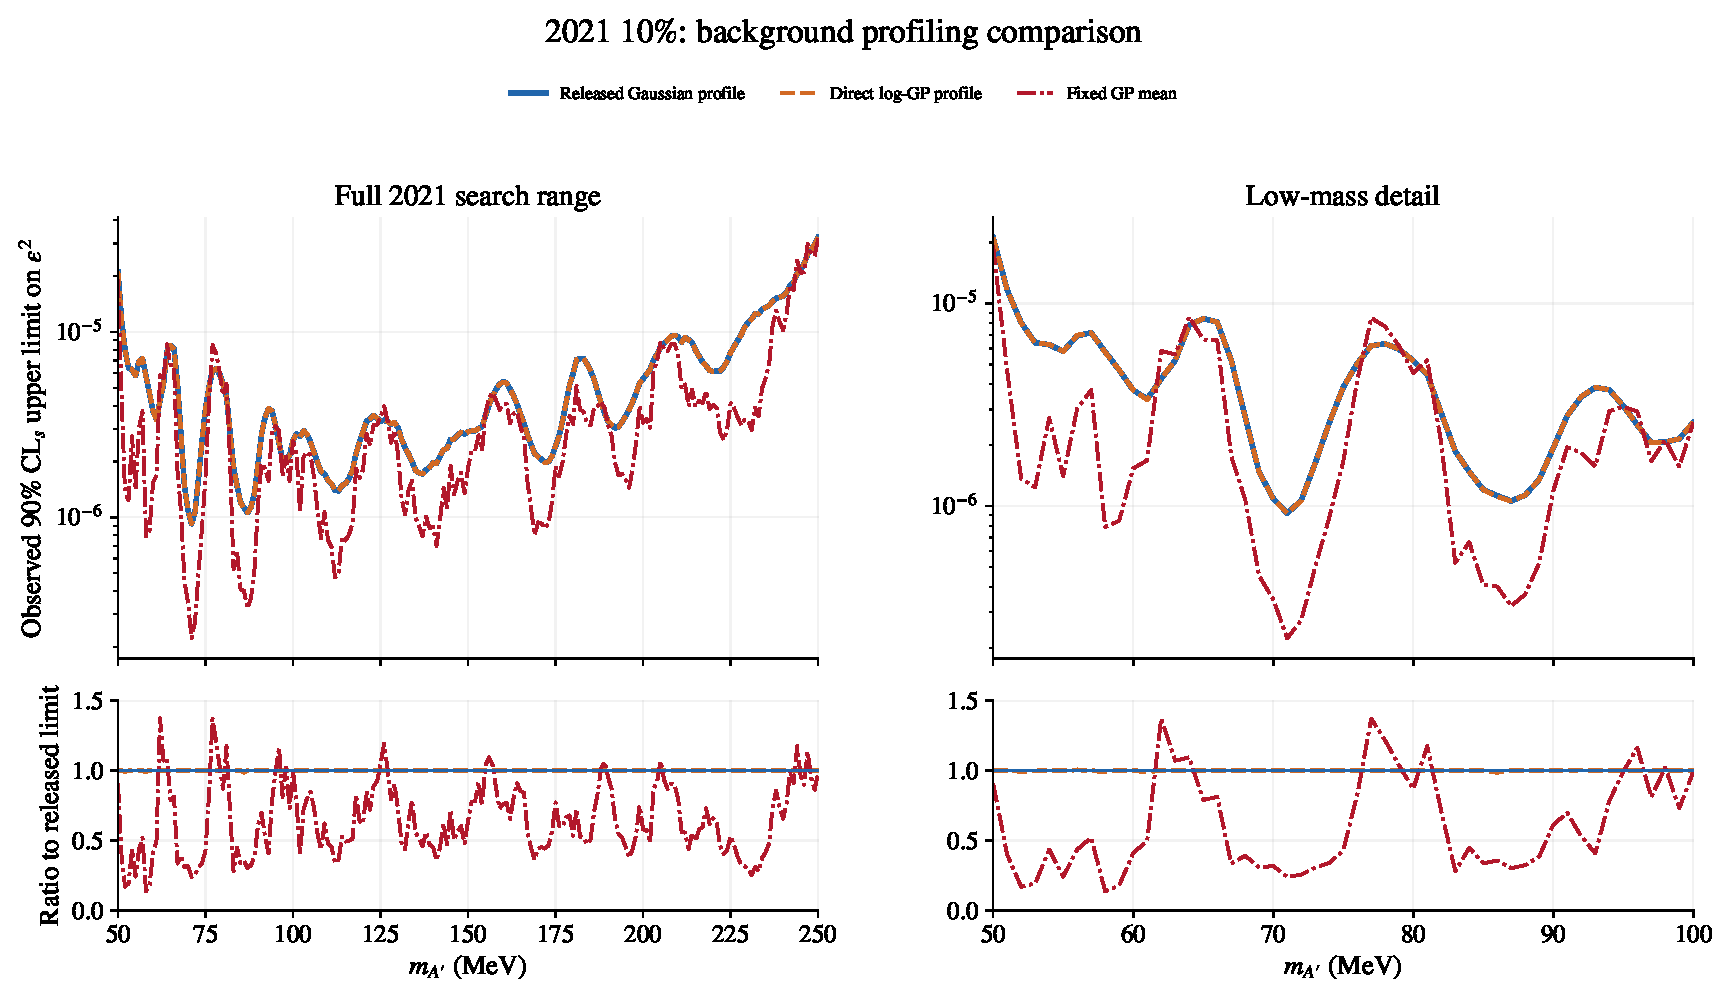
\includegraphics[width=0.96\linewidth]{../figures/v5_profile_background_comparison.pdf}
\caption{Controlled comparison of observed 2021 10\% upper limits using the
nominal correlated Gaussian background profile, a positive log-GP profile,
and a fixed GP mean. All curves use the same observed counts and frozen
analysis settings. The dimuon branching correction is applied once above
threshold. The fixed-mean curve omits background-estimation uncertainty;
its smaller uncalibrated limit is assessed against the injection and
calibration studies below. Adapted from Fig.~1 of the v4.9.13 calibration report.}
\label{v5-fig:profile-comparison}
\end{figure}

\subsection{What the signal injections establish}
\label{v5-sec:profile-injections}
The dedicated comparison generated 500 spectra at each of six masses,
65, 71, 78, 100, 182 and 231~MeV, for each tested background construction
and injection $A_{\rm true}=0,2\sigma_{\rm ref},5\sigma_{\rm ref}$.
Here $\sigma_{\rm ref}$ is the profiled Fisher reference error fixed before
generation. Thus a five-reference-error injection means a fixed physical
event yield within that ensemble, rather than a guarantee of a measured
$5\sigma$ significance. Both methods fit the same spectra and physical
signals; different injection strengths use separate ensembles.

Three constructions separate different questions. A known-background
control tests the fitting machinery when the fixed assumption is exact.
A second construction varies the background with the nominal GP covariance
and tests whether that uncertainty is correctly propagated. A third
fluctuates a complete smooth spectrum and retrains the sidebands, including
signal tails outside the moving mask. The latter spectrum was obtained
from data outside 60--86~MeV using the frozen 66~MeV kernel. It is a selected
response diagnostic, and does not independently define the physical
background family.

\begin{figure}[htbp]\centering
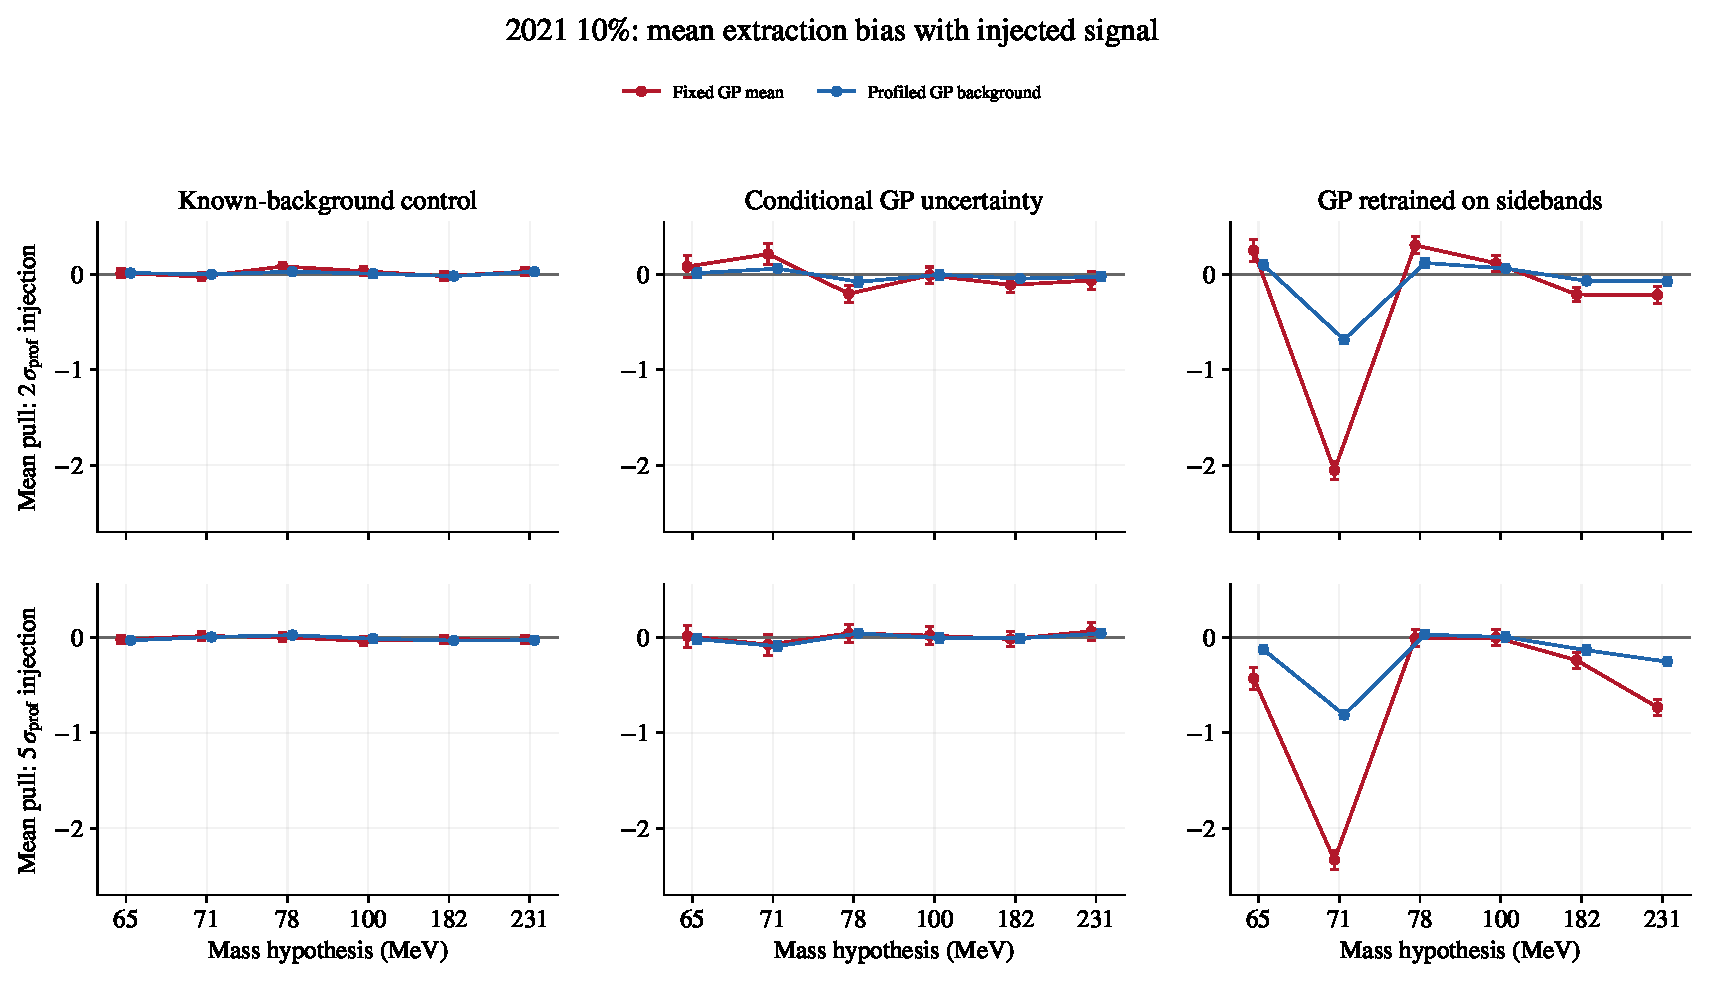
\includegraphics[width=0.96\linewidth]{../figures/v5_profile_injected_bias.pdf}
\caption{Mean signal-extraction pull for injections of
$2\sigma_{\rm ref}$ and $5\sigma_{\rm ref}$, where the profiled Fisher
reference error fixes the event yield before generation. Each
mass--strength--background cell contains 500 spectra, shared by the fixed
and profiled methods. Pull denotes
$(\widehat A-A_{\rm true})/\widehat\sigma_A$; bars are Monte Carlo errors
on its mean. At 71~MeV, a signal injected at 71~MeV into the retrained
smooth-background construction has mean pull $-2.33$ for the fixed fit
and $-0.81$ for the profiled fit at the stronger injection. Profiling reduces
this conditional offset below one fitted standard error, but the
associated exclusion test still fails. Adapted from Fig.~9 of the
v4.9.13 calibration report.}
\label{v5-fig:profile-bias}
\end{figure}

When the nominal GP uncertainty is present in generation, the fixed fit
has background-only pull widths of 1.85--2.65 and excludes the true stronger
injection in 22.0--32.2\% of trials. The corresponding profiled exclusion
fractions are 8.2--12.2\%. Profiling is therefore the better motivated
baseline for 2021. The retrained 71~MeV example also identifies a limitation:
the fixed and profiled fits exclude the true stronger yield in 349/500
and 145/500 trials, respectively. A mean pull smaller than one does not
by itself ensure a valid 90\% exclusion rule.

The nominal analysis uses profiled asymptotic $CL_s$ limits. The
signal-recovery tests favor profiling, but the calibration study shows
that the resulting probabilities can still depend strongly on the
background shape. Appendix~\ref{v5-sec:calibration} compares the
asymptotic and empirical probability calculations, including the large
differences in part of the 2016 scan.
